\documentclass[10pt,a4paper,sans]{moderncv}
\moderncvstyle{banking}
\moderncvcolor{black}
\nopagenumbers{}

\usepackage[utf8]{inputenc}
\usepackage[top=0.15cm, bottom=0cm, left=0.30cm, right=0.30cm]{geometry}
\usepackage{ragged2e}
\usepackage{multicol}
\usepackage{enumitem}
\usepackage{amssymb}
\usepackage{fontawesome5}
\usepackage{xcolor}
\usepackage{hyperref}
\hypersetup{colorlinks=true, urlcolor=blue}

% Custom cventry
\newcommand*{\customcventry}[7][.10em]{%
\begin{tabular}{@{}l}
    {\bfseries #4} \\
    {\itshape #3}
\end{tabular}
\hfill
\begin{tabular}{l@{}}
    {\bfseries #5} \\
    {\itshape #2}
\end{tabular}
\ifx&#7&%
\else{\\
\begin{minipage}{\maincolumnwidth}%
    \footnotesize#7%
\end{minipage}}\fi%
\par\addvspace{#1}
}

\begin{document}

% Ultra-compact header: photo left (not in margin), title/info centered and bigger
\hspace*{0.03\textwidth}% less horizontal space before photo (10% bump back)
\begin{minipage}[c]{0.13\textwidth}
  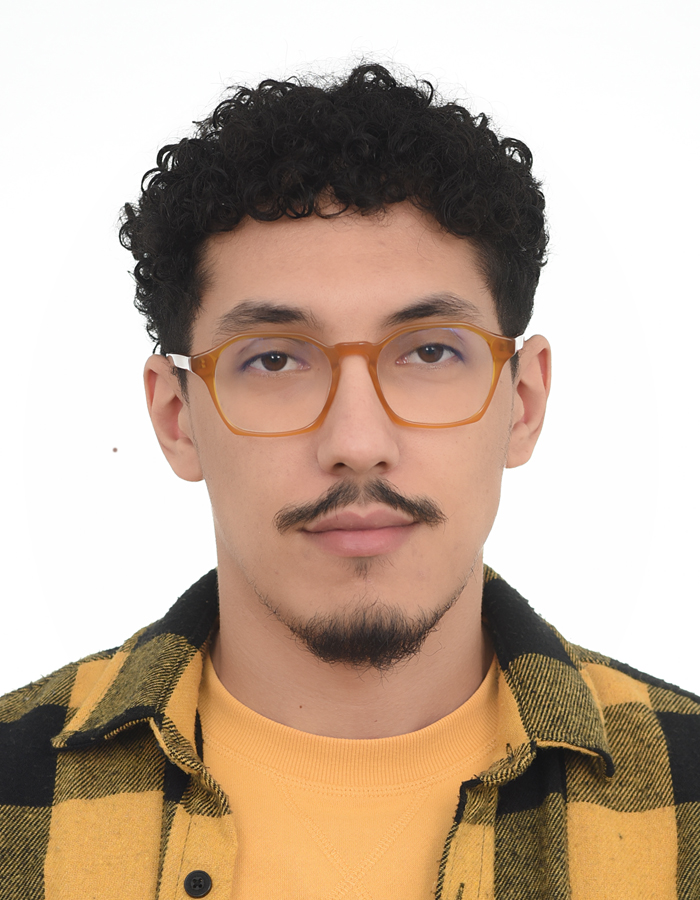
\includegraphics[width=0.85\linewidth]{images/ahmed.jpg}
\end{minipage}%
\hfill
\begin{minipage}[c]{0.84\textwidth}
  \begin{center}
    {\fontsize{20}{22}\selectfont\textbf{Ahmed MAKROUM}}\\[0.7em]
    {\fontsize{13.2}{15.4}\selectfont Data Engineer \& Full-Stack Web/Mobile Developer} \\[0.5em]
    {\fontsize{10.5}{12.3}\selectfont
      \faMobile\enspace +212 6 64 71 62 19 \quad
      \faEnvelope\enspace ahmedmakroum3@gmail.com \quad
      \faHome\enspace Casablanca, Morocco \\
      \faLinkedin\enspace \href{https://www.linkedin.com/in/ahmed-makroum/}{in/ahmed-makroum} \quad
      \faGithub\enspace \href{https://github.com/ahmedmakroum}{github.com/ahmedmakroum}\quad
      \faGlobe\enspace \href{https://makroum.website}{makroum.website}
    }\\[1em]
  \end{center}
\end{minipage}
\vspace{-17pt}

% PROFILE
\section{\fontsize{11}{12.1}\selectfont Profile}
\vspace{-6pt}
State Engineer specialized in data engineering and full-stack development. Experienced in creating data pipelines, developing web applications, and utilizing cloud platforms. I am seeking a position where I can design and develop innovative projects, enhance system performance, and collaborate with technical teams to create impactful solutions.
% EXPERIENCE
\vspace{-17pt}
{\renewcommand{\labelitemi}{\raisebox{0.2ex}{\scalebox{1.15}{$\bullet$}}} % +15% size for bullets here only
\section{\fontsize{11}{12.1}\selectfont Experience}
\vspace{-3pt}

\customcventry{03/2025 ‐ 08/2025}{\href{https://www.allianz.ma}{Allianz Morocco}}{Data Engineer}{}{}{
\begin{itemize}[leftmargin=0.8cm, itemsep=-2pt, topsep=0pt, partopsep=0pt, parsep=0pt]
\fontsize{10.5}{12.3}\selectfont
\item Designed and deployed data pipelines (NiFi, Spark) for extraction, cleaning, and loading from internal insurance systems, enabling automation of previously manual processes.
\item Integrated fragmented sources into a PostgreSQL data warehouse, consolidating multiple business streams.
\item Created dashboards with Metabase, facilitating data access for business users and enabling direct visualization of key indicators.
\item Developed and maintained a web application for health claims management using a microservices architecture (Spring Boot, Next.js), with fine-grained role management and secure authentication, used daily by business teams.
\end{itemize}}

\customcventry{06/2024 ‐ 08/2024}{\href{https://boti.education/}{BOTI School}}{Data Engineer}{}{}{
\begin{itemize}[leftmargin=0.8cm, itemsep=-2pt, topsep=0pt, partopsep=0pt, parsep=0pt]
\fontsize{10.5}{12.3}\selectfont
\item Developed a distributed ETL pipeline with Apache Beam on Google Cloud to process millions of user logs.
\item Structured data from GCP buckets, enabling reliable behavioral analysis.
\item Designed automated dashboards via Looker, adopted by the team to improve strategic decision-making.
\end{itemize}}

\customcventry{06/2023 ‐ 08/2023}{\href{https://6solutions.com/}{6solutions}}{Web and Mobile Developer}{}{}{
\begin{itemize}[leftmargin=0.8cm, itemsep=-2pt, topsep=0pt, partopsep=0pt, parsep=0pt]
\fontsize{10.5}{12.3}\selectfont
\item Developed a multi-service consulting platform (legal, medical, financial).
\item Front-end built with Angular, back-end with Spring Boot.
\item Designed and deployed the mobile version of the application using Flutter.
\end{itemize}}

\customcventry{07/2022 ‐ 08/2022}{\href{https://estatmar.ma/}{Finso}}{Game Developer}{}{}{%
\begin{itemize}[leftmargin=0.8cm, itemsep=-2pt, topsep=0pt, partopsep=0pt, parsep=0pt]
\fontsize{10.5}{12.3}\selectfont
\item Developed an educational game for children to introduce basic management and strategy concepts.
\item Built using Unity with interactive gameplay, polished animations, and a user interface tailored for a young audience.
\end{itemize}}}
}

% PROJECTS
\vspace{-14pt}
\section{\fontsize{11}{12.1}\selectfont Projects}
\vspace{-4pt}
\begin{itemize}[leftmargin=0.3cm, itemsep=-2pt, topsep=0pt, partopsep=0pt, parsep=0pt]
    \item \textbf{News Pipeline}: Multi-source scraping orchestrated with Airflow, streaming transformation with Kafka, LLM enrichment (summaries + validation), Prometheus monitoring, Cassandra storage. (Python, Kafka, LLM API, Airflow, Cassandra)
    \item \textbf{Website Log Analysis Pipeline}: Real-time collection of website event logs (clicks, page views), ingestion orchestration with Cloud Composer, data storage and analysis in BigQuery, creation of a dashboard for traffic and error tracking. (Cloud Composer, GCP, BigQuery, Python)
    \item \textbf{Morocco Product Price Tracking}: Daily scraping of product prices (food, electronics, etc.), PostgreSQL storage, comparison dashboards by city/product, inflation alerts. (Python, Airflow, Metabase, PostgreSQL)
    \item \textbf{JobTrack – Application Tracking}: Web application for managing job applications (resumes, statuses, notes) with Cloudinary storage, real-time search, and statistics visualization. (Next.js, Tailwind, MongoDB, Cloudinary)
\end{itemize}

% EDUCATION
\vspace{-17pt}
\section{\fontsize{11}{12.1}\selectfont Education}
\vspace{-4pt}
\customcventry{2020 -- 2025}{\href{https://emsi.ma}{\textbf{EMSI – Moroccan School of Engineering Sciences}}}{Master’s degree in Software Engineering and Networks \\ (IT Methods Applied to Business Management)}{}{}{}
\customcventry{Jul. 2024 ‐ Sep. 2024}{\href{https://www.alxafrica.com}{\textbf{ALX Academy}}}{Diploma in Artificial Intelligence and Prompt Engineering}{}{}{ALX AiCE – AI Fundamentals}

% CERTIFICATIONS
\vspace{-18pt}
\section{\fontsize{11}{12.1}\selectfont Certifications}
\vspace{-5pt}
\textit{Certifications obtained via Coursera.}
\begin{itemize}[leftmargin=0.3cm, itemsep=-2pt, topsep=0pt, partopsep=0pt, parsep=0pt]
    \item \textbf{\href{https://www.coursera.org/account/accomplishments/verify/G178XXP17WQA}{Machine Learning with Python}} (IBM)
    \item \textbf{\href{https://www.coursera.org/account/accomplishments/records/M5RKGX36BAVA}{IBM Data Engineering}} (IBM)
    \item \textbf{\href{https://google.com}{Building Scalable Java Microservices with Spring Boot and Spring Cloud}} (Google Cloud)
    \item \textbf{\href{https://www.coursera.org/account/accomplishments/verify/EK5SJM3YM7PX}{Introduction to Big Data with Spark and Hadoop}} (IBM)
    \item \textbf{\href{https://www.coursera.org/account/accomplishments/specialization/B4RCUAYCUG49}{Python for Everybody Specialization}} (University of Michigan)
    \item \textbf{\href{https://www.coursera.org/account/accomplishments/records/G867SJLRFQS2}{Google Business Intelligence}} (Google)
\end{itemize}

% SKILLS
\vspace{-18pt}
\section{\fontsize{11}{12.1}\selectfont Skills}
\vspace{-6pt}
\begin{itemize}[leftmargin=0.3cm, itemsep=-2pt, topsep=0pt, partopsep=0pt, parsep=0pt]
  \item \textbf{Data Engineering}: ETL (NiFi, Airflow), Big Data (Hadoop, Spark), Kafka, PostgreSQL, Cassandra, GCP, AWS
  \item \textbf{Programming}: Python, SQL, Java, TypeScript
  \item \textbf{Web/Mobile}: React, Next.js, Flutter, Spring Boot, REST APIs
  \item \textbf{DevOps and Cloud}: Docker, Kubernetes, Git, CI/CD, Linux
  \item \textbf{Visualization}: Metabase, Superset, Power BI
  \item \textbf{Soft Skills}: Teamwork, communication, adaptability, problem-solving
\end{itemize}

% LANGUAGES
\vspace{-18pt}
\section{\fontsize{11}{12.1}\selectfont Languages}
\vspace{-17pt}
\begin{multicols}{2}
\begin{itemize}[leftmargin=0.3cm, itemsep=-2pt, topsep=0pt, partopsep=0pt, parsep=0pt]
    \item English – Fluent
    \item French – Fluent
    \item Arabic – Native
    \item Spanish – Basic
\end{itemize}
\end{multicols}

% FOOTER
\vspace{-20pt}
\begin{center}
    {\fontsize{9}{11}\selectfont\color{gray}
    For more about my work, visit my~
    \faLinkedin~\href{https://www.linkedin.com/in/ahmed-makroum/}{LinkedIn}~or~\faGithub~\href{https://github.com/ahmedmakroum}{GitHub}.}
\end{center}

\end{document}